\begin{frame}\begin{center}
		\LARGE\textbf{Job market signaling}
\end{center}\end{frame}
%-------------------------------------------------------------------------------
%-------------------------------------------------------------------------------
\begin{frame}

We study the seminal model presented in \citeA{Spence.1973}.
\begin{itemize}\setlength\itemsep{1em}
\item There are two groups $j \in\{H, L\}$ in the population facing one employer, where  $h_{i\in\{L, H\}}$ denotes the respective level of productivity.
\item Group $H$ is a proportion $q_H$ in the population.
\item Education $y$ is measured by an index $y$ of level and achievement and is subject to individual choice.
\item Education costs are both monetary and psychic and differ by group $c_{i\in\{L, H\}}$.
\end{itemize}

\end{frame}
%-------------------------------------------------------------------------------
%-------------------------------------------------------------------------------
\begin{frame}\begin{figure}[htp]\centering
\caption{Informational feedback}
\scalebox{0.35}{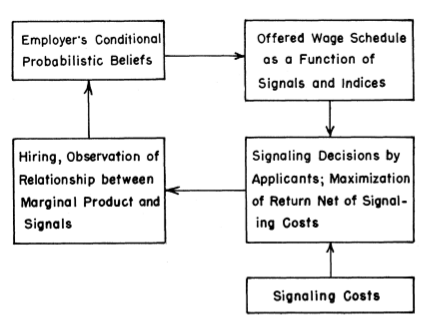
\includegraphics{fig-model-spence-informational-feedback.png}}
\end{figure}\end{frame}
%-------------------------------------------------------------------------------
%-------------------------------------------------------------------------------
\begin{frame}

We explore the following parameterized version.

\begin{align*}\begin{array}{l@{\qquad}l}
	h_L = 1   & h_H = 2 \\
	c_L = y   & c_H = \tfrac{1}{2}\,y \\
\end{array}\end{align*}

\end{frame}
%-------------------------------------------------------------------------------
%-------------------------------------------------------------------------------
\begin{frame}\begin{figure}[htp]\centering
\caption{Benefit of education}
\scalebox{0.35}{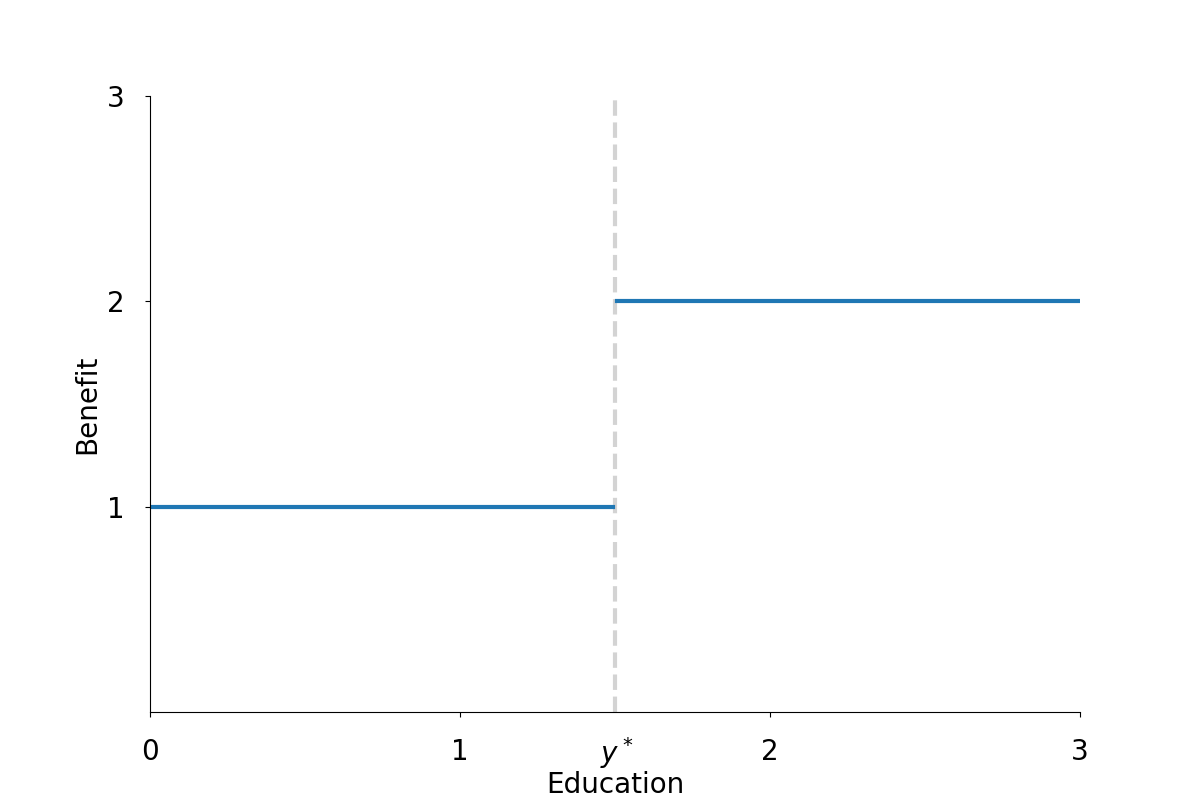
\includegraphics{fig-model-spence-benefit}}
\end{figure}\end{frame}
%-------------------------------------------------------------------------------
%-------------------------------------------------------------------------------
\begin{frame}\begin{figure}[htp]\centering
\caption{Cost of education}
\scalebox{0.35}{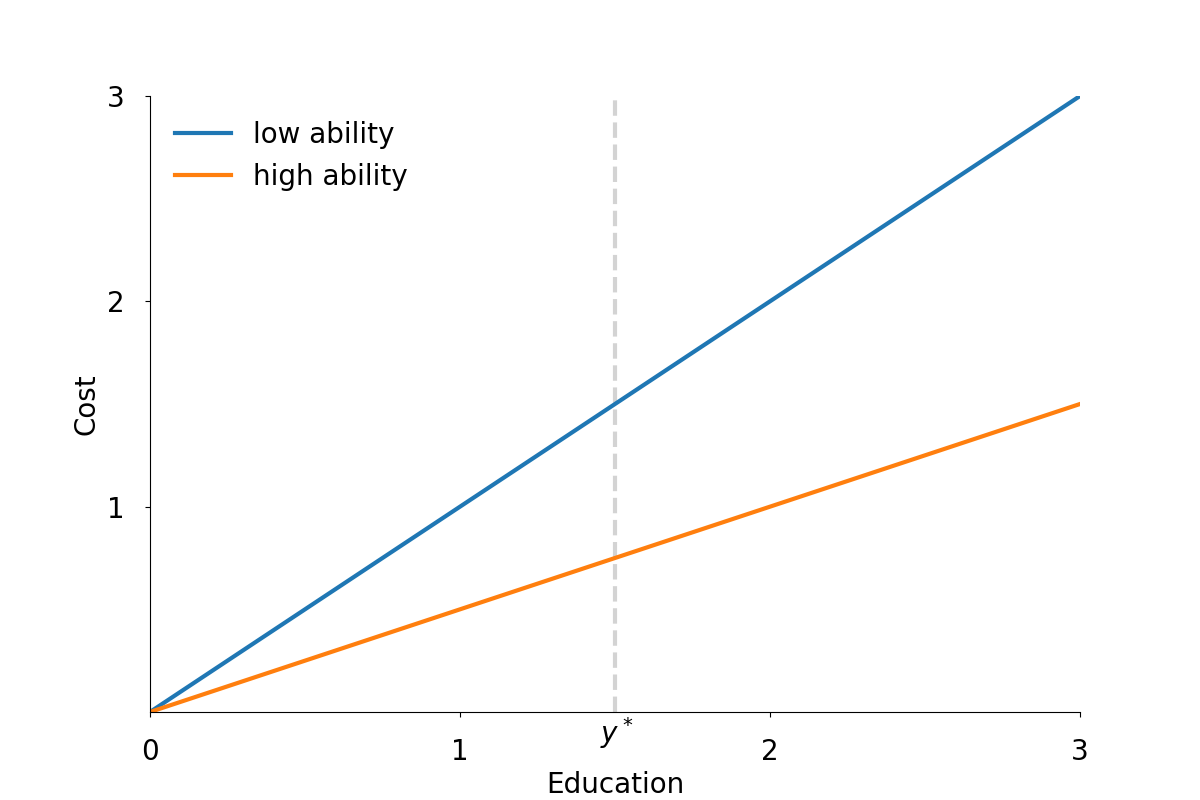
\includegraphics{fig-model-spence-cost}}
\end{figure}\end{frame}
%-------------------------------------------------------------------------------
%-------------------------------------------------------------------------------
\begin{frame}\begin{figure}[htp]\centering
\caption{Surplus of education I}
\scalebox{0.35}{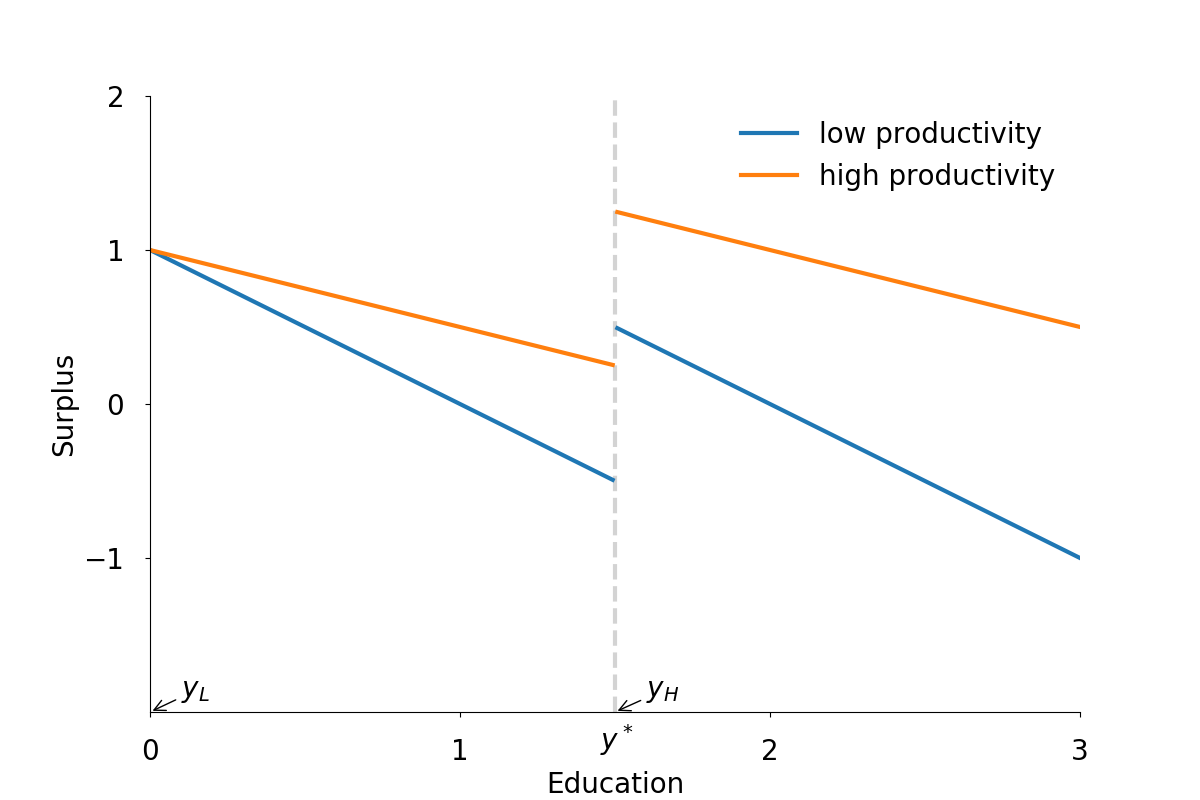
\includegraphics{fig-model-spence-surplus-base}}
\end{figure}\end{frame}
%-------------------------------------------------------------------------------
%-------------------------------------------------------------------------------
\begin{frame}
\begin{itemize}\setlength\itemsep{1em}
\item For $y^* = 1.5$ the employer's beliefs are confirmed. More generally, $L$ chooses $y_L = 0$ if $1 > 2 - y^*$ and $H$ acquires $y_H = y^*$ provided that $2 - 0.5\,y^* > 1$.
\item Beliefs are confirmed provided that the following holds:
	\begin{align*}
	1 < y^* < 2
	\end{align*}
\end{itemize}
\end{frame}
%-------------------------------------------------------------------------------
%-------------------------------------------------------------------------------
\begin{frame}\begin{figure}[htp]\centering
\caption{Surplus of education II}
\scalebox{0.35}{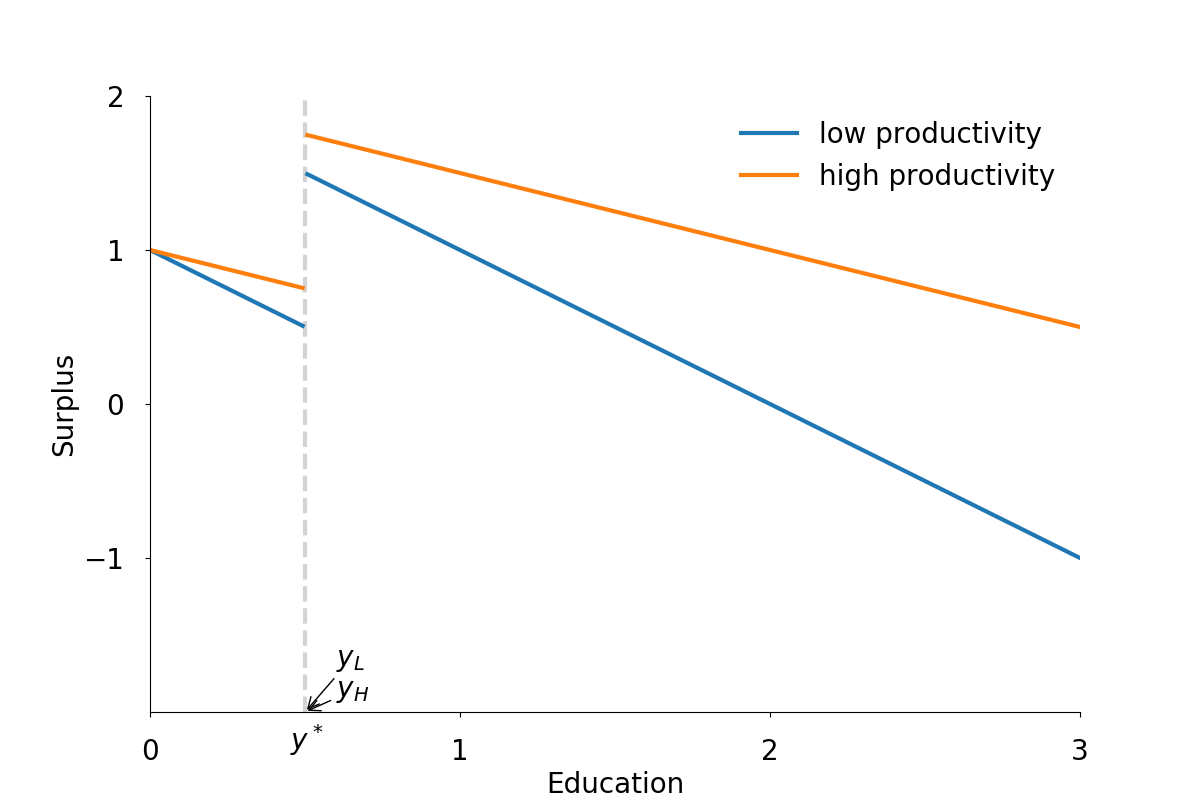
\includegraphics{fig-model-spence-surplus-low}}
\end{figure}\end{frame}
%-------------------------------------------------------------------------------
%-------------------------------------------------------------------------------
\begin{frame}\begin{figure}[htp]\centering
\caption{Surplus of education III}
\scalebox{0.35}{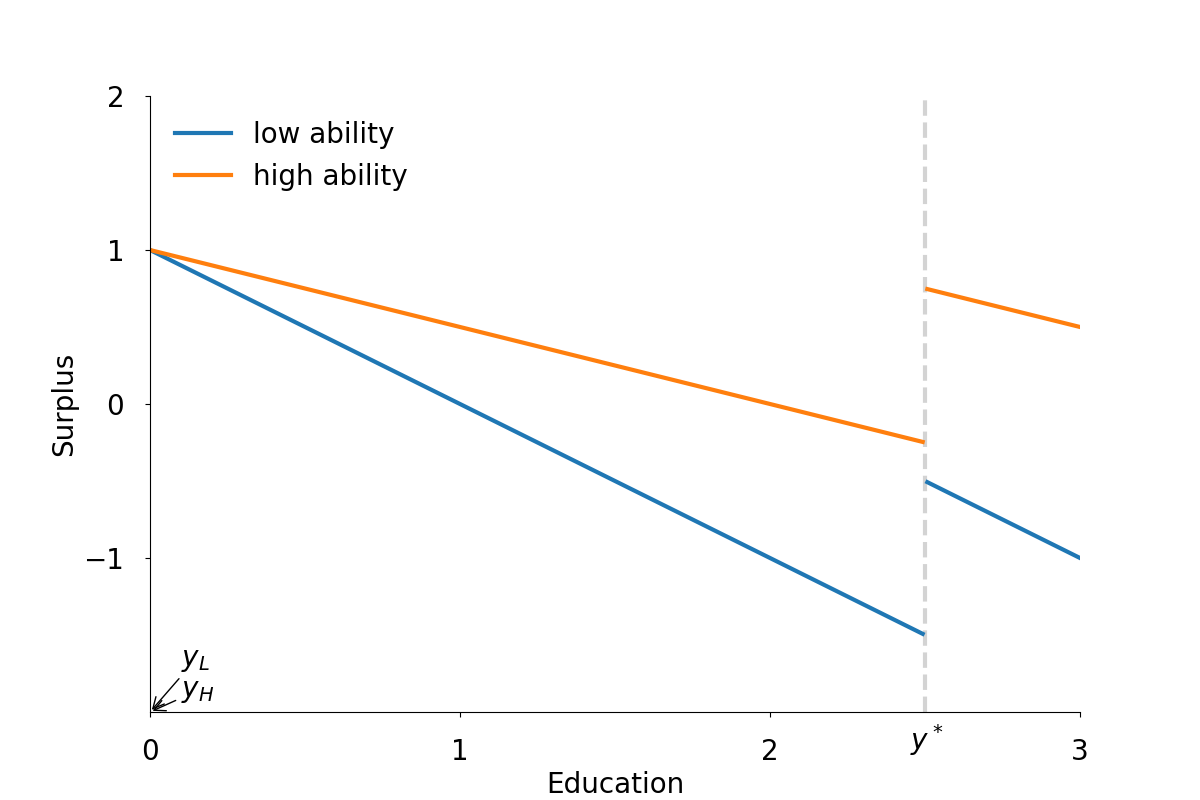
\includegraphics{fig-model-spence-surplus-high}}
\end{figure}\end{frame}
%-------------------------------------------------------------------------------
%-------------------------------------------------------------------------------
\begin{frame}
\begin{itemize}\setlength\itemsep{1em}
\item From the outside, education appears to be productive and is for the individual. However, there is no real effect on the marginal product.
\end{itemize}
\end{frame}
%-------------------------------------------------------------------------------
%-------------------------------------------------------------------------------
\begin{frame}
\begin{itemize}\setlength\itemsep{1em}
\item In the absence of signaling, both groups are paid the unconditional expected marginal product.
	\begin{align*}
	   &  q_L\times 1 + (1 - q_L) \times 2
	\end{align*}
\end{itemize}
\end{frame}
%-------------------------------------------------------------------------------
%-------------------------------------------------------------------------------
\begin{frame}
\begin{itemize}\setlength\itemsep{1em}
\item It depends on the share of low ability individuals whether high ability individuals actually prefer a no-signaling case. The surplus is determined as follows:
	\begin{align*}\begin{array}{ll}
	\text{signaling}    & 2 - \tfrac{1}{2} y^* \\
	\text{no-signaling} & 2 - q_L
	\end{array}\end{align*}
\item High ability individual prefer the signaling case as long as $y^* \leq 2 q_L$.
\end{itemize}
\end{frame}
%-------------------------------------------------------------------------------
%-------------------------------------------------------------------------------
\begin{frame}\begin{figure}[htp]\centering
\caption{Market structure}
\scalebox{0.35}{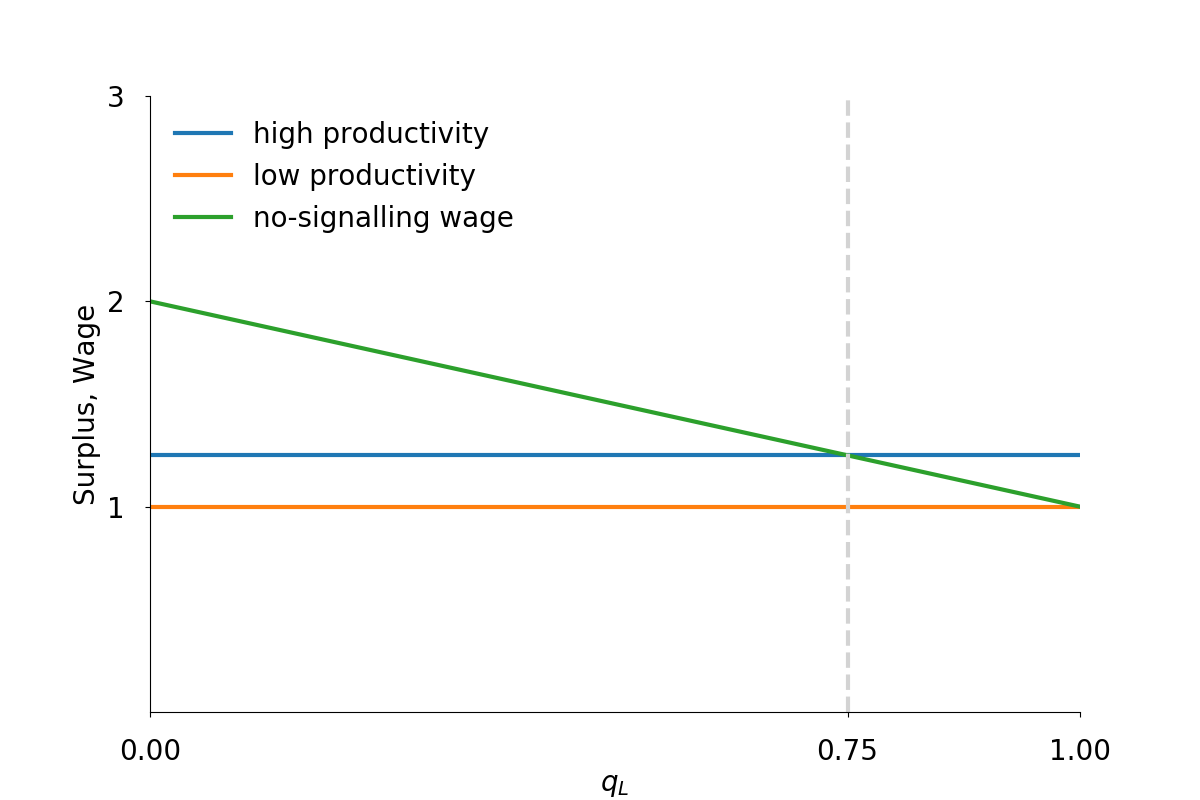
\includegraphics{fig-model-spence-market-structure}}
\end{figure}\end{frame}
%-------------------------------------------------------------------------------
%-------------------------------------------------------------------------------
\begin{frame}
\begin{itemize}\setlength\itemsep{1em}
\item The ability to signal has a detrimental effect on low ability workers, while the consequences are ambiguous for high ability workers.

\item High ability workers benefit from their ability to send a signal if their proportion is sufficiently small with respect to the ability gap to low ability individuals.
\end{itemize}
\end{frame}
